
%TODO refer to the error analysis instead to show that these types of errors are reduced by BSC-Seq.
% \begin{figure*}[t]
% \centering
% \subfloat[Annotator accuracy bias]{
%   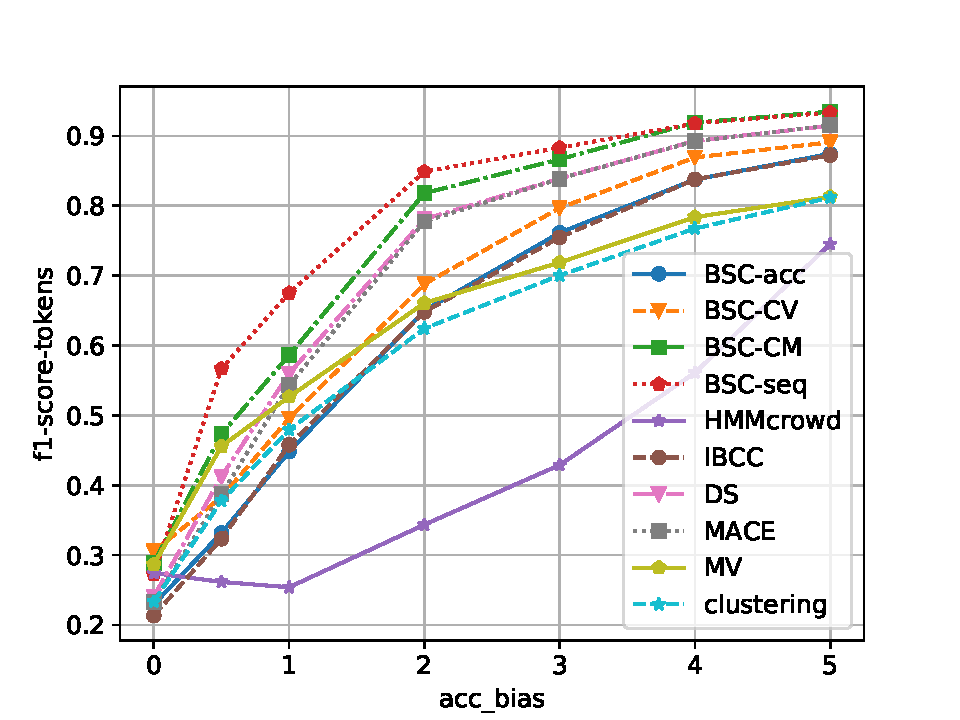
\includegraphics[width=0.505\columnwidth, clip=True, trim=0 20 45 40]{figures/synthetic/acc_bias_exp/plot_f1-score-tokens}
% }
% \subfloat[Short span bias]{
%   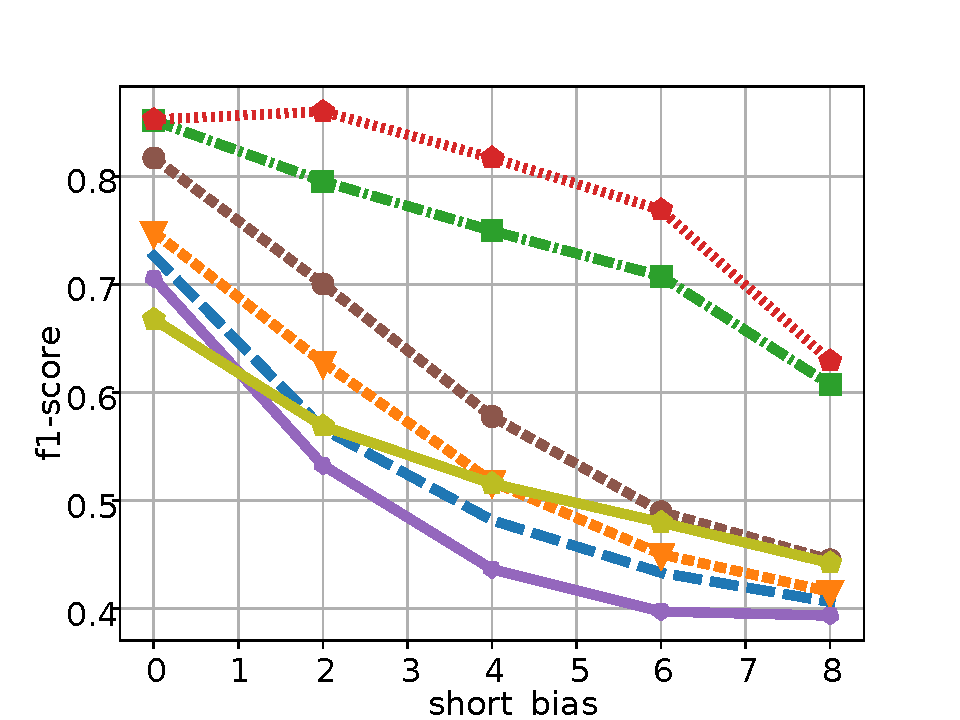
\includegraphics[width=0.485\columnwidth, clip=True, trim=24 18 40 40]{figures/synthetic/short_bias_exp/plot_f1-score-tokens}
% }
% \subfloat[Missed span bias]{
%   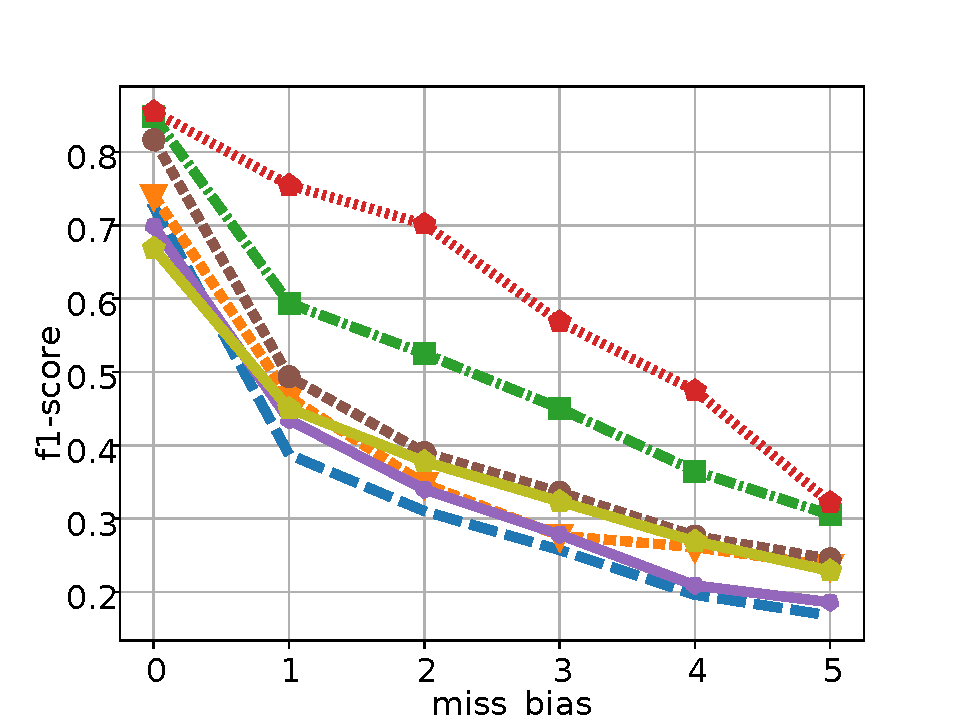
\includegraphics[width=0.485\columnwidth, clip=True, trim=24 18 45 40]{figures/synthetic/class_bias_exp/plot_f1-score-tokens}
% }
% % \subfloat[Crowd size]{
% %   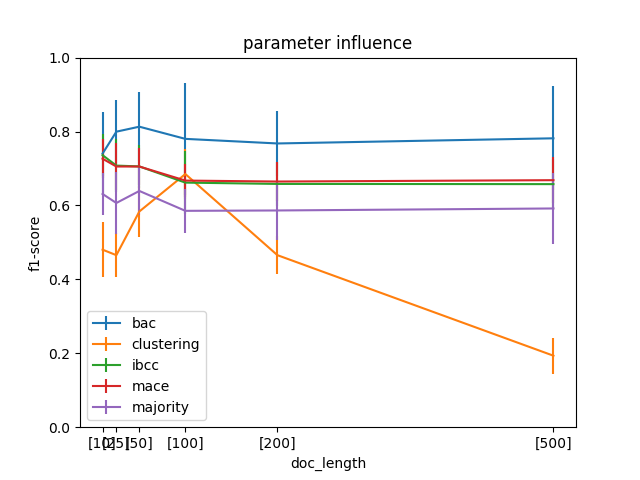
\includegraphics[width=0.2\textwidth, clip=True, trim=0 10 0 27]{figures/synthetic/acc_bias_exp/plot_f1-score.png}
% % }
% \subfloat[
% Good workers out of 10 %a crowd of , where the rest are random.
% ]{
%   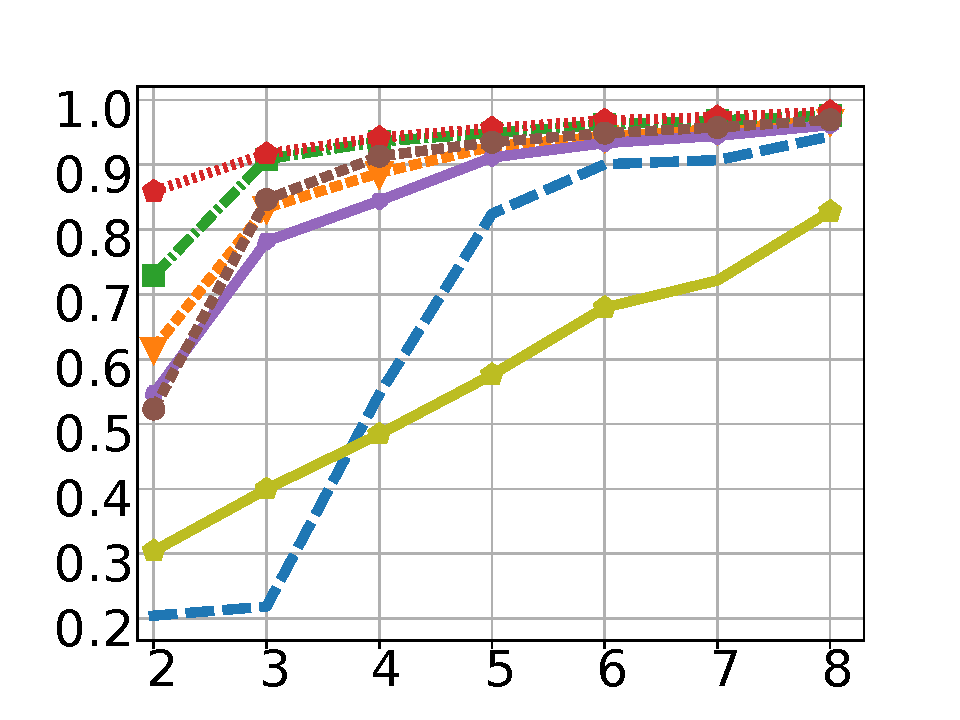
\includegraphics[width=0.485\columnwidth, clip=True, trim=24 18 40 40]{figures/synthetic/group_ratio_exp/plot_f1-score-tokens}
% }
% \caption{F1 scores with simulated annotators. Each plot shows the effect of varying one characteristic.}
% \label{fig:simulated}
% \end{figure*}

\section{Experiments}\label{sec:expts_all}

\begin{table}[t]
\small
\centering
\setlength{\tabcolsep}{3pt}
\begin{tabular}{l l l l l l l l} \toprule
data & \multicolumn{3}{l}{\#sentences or docs} & %#tokens & 
\multicolumn{2}{l}{\#annotators} & \#gold & span \\ %\multicolumn{2}{l}{span length}  \\
-set & total & dev & test
& %/sent. & 
total & /doc & spans & length \\ %mean & std.  \\
\toprule
NER & 6,056 & 2,800 & 3,256 & %13 & 
47 & 4.9 & 21,612 % mean per type (std) 5403 (1376) 
& 1.51 \\%& 0.75 \\
PICO & 9,480 & 191 & 191 & %150 & 
312 & 6.0 & 700 & 7.74 \\%& 7.38  \\
ARG & 8,000 & 60 & 100 & 105 & 5 & 73 &  17.52 \\
 \bottomrule
\end{tabular}
\caption{
%Numbers of sentences, annotators, and spans for datasets used in our experiments. Sentences with crowd all have crowdsourced labels. Only dev and test sentences have gold sequence labels.
Dataset statistics. Span lengths are means.
}
\label{tab:datasets}
\end{table}
 
% TODO: write about the hyper-parameters?
\begin{table*}
\small
\centering
\nprounddigits{1}
\npdecimalsign{.}
\setlength{\tabcolsep}{4pt}
\begin{tabular}{l l l l r@{\hskip 0.8cm} l l l r@{\hskip 0.8cm} l l l r }
\toprule
& \multicolumn{4}{l}{NER} & \multicolumn{4}{l}{PICO} & \multicolumn{3}{l}{ARG} \\ 
%& \multicolumn{4}{l}{ARG: relaxed} \\
& \text{Prec.} &  \text{Rec.} & \text{F1} & \text{CEE} & 
\text{Prec.} & \text{Rec.} & \text{F1} & \text{CEE} & 
%\text{Prec.} & \text{Rec.} & \text{F1} &
\text{Prec.} & \text{Rec.} & \text{F1} & \text{CEE} 
\\ \toprule
Best worker & 
76.4 & 60.1 & 67.3 & 17.1 & 
64.8 & 53.2 & 58.5 & 17.0 & 
62.7 & 57.5 & 60.0 & %79.2 & 76.4 & 77.8 & 
44.20 
\\
Worst worker & 
55.7 & 26.5 & 35.9 & 31.9 &
50.7 & 52.9 & 51.7 & 41.0 & 
25.5 & 19.2 & 21.9 & %80.0 & 41.3 & 54.5 & 
70.33
\\ \midrule
MV & 
79.9 & 55.3 & 65.4 & 6.24 &
82.5 & 52.8 & 64.3 & 2.55 & 
40.0 & 31.5 & 34.8 & %88.2 & 60.1 & 71.5 & 
14.03
\\ 
MACE & 
74.4 & 66.0 & 70.0 & 1.01 & 
25.4 & 84.1 & 39.0 & 58.2 & 
31.2 & 32.9 & 32.0 & %81.0 & 60.8 & 69.4 & 
2.62
\\ 
DS & 
79.0 & 70.4 & 74.4 & 2.80 & 
71.3 & 66.3 & 68.7 & 0.44 & 
% new implementation -- bad init? 34.6 & 75.1 & 47.4 & 0.40 &
45.6 & 49.3 & 47.4 & %80.3 & 76.4 & 78.3 & 
0.97
\\ 
IBCC & 
79.0 & 70.4 & 74.4 & \textbf{0.49} & 
72.1 & 66.0 & 68.9 & \textbf{0.27} &
44.9 & 47.9 & 46.4 & %80.3 & 76.4 & 78.3 & 
\textbf{0.85}
\\ \midrule
HMM-crowd & 
80.1 & 69.2 & 74.2 & 1.00 & 
75.9 & 66.7 & 71.0 & 0.99 &
43.5 & 37.0 & 40.0 & %87.0 & 61.8 & 72.2 & 
3.38
\\ 
\midrule
BSC-acc & 
\textbf{83.4} & 54.3 & 65.7 & 0.96 &
\textbf{89.4} & 45.2 & 60.0 & 1.59 &  
36.9 & 32.9 & 34.8 & %87.7 & 59.2 & 70.7 & 
6.47
\\ 
BSC-spam &
67.9 & 74.1 & 70.9 & 0.89 &
46.7 & \textbf{84.4} & 60.1 & 1.98 & 
55.7 & 53.4 & 54.5 & %85.8 & 77.3 & 81.3 & 
2.80
\\ 
BSC-CV & 
83.0 & 64.6 & 72.6 & 0.93 &
74.9 & 67.2 & 71.1 & 0.84 & 
37.9 & 34.2 & 36.0 & %87.2 & 60.5 & 71.5 &
 4.73
 \\ 
BSC-CM & 
79.9 & 72.2 & 75.8 & 1.46 & 
60.1 & 78.8 & 68.2 & 1.49 & 
\textbf{56.0} & 57.5 & 56.8 & %80.3 & 79.1 & 79.7 & 
3.76 
\\ 
BSC-seq & 
80.3 & \textbf{74.8} & \textbf{77.4} & 0.65 & 
70.4 & 75.3 & \textbf{72.8} & 0.53 & 
54.4 & \textbf{67.1} & \textbf{60.1} & %70.2 & 86.5 & 77.5 &
 3.26
\\ \midrule
BSC-CM-notext & 
74.7 & 69.7 & 72.1 & 1.48 & 
62.7 & 74.8 & 68.2 & 1.32 & 
55.1 & 58.9 & 57.0 & 2.75
\\
BSC-CM$\backslash\bs T$ & 
80.0 & 73.0 & 76.3 & 0.99 &
65.8 & 66.7 & 66.2 & 0.28 &
52.9 & 49.3 & 51.1 & 1.69
 \\
BSC-seq-notext & 
81.3 & 71.9 & 76.3 & 0.52 & 
81.2 & 59.2 & 68.5 & 0.73 &
36.9 & 52.0 & 43.2 & 5.64 
\\ 
BSC-seq$\backslash\bs T$ & 
64.2 & 44.4 & 52.5 & 0.77 &
51.2 & 70.4 & 59.8 & 1.04 &
0.11 & 0.05 & 0.07 & 6.38
\\
\bottomrule 
\end{tabular}
\caption{Aggregating crowdsourced labels: estimating true labels for documents labelled by the crowd.}
\label{tab:aggregation_results}
\npnoround
\end{table*}

\paragraph{Datasets. }\label{sec:expts}

We compare BSC to alternative methods on three NLP datasets
%to test performance in passive and active learning scenarios, 
%analyze errors, and
%visualize the learned annotator models.
containing both crowdsourced and gold sequential annotations.
\emph{NER}, the CoNLL 2003 named-entity recognition dataset~\cite{tjong2003introduction},
which contains gold labels for four named entity categories (PER, LOC, ORG, MISC),
with crowdsourced labels provided by \cite{rodrigues2014sequence}.
\emph{PICO}~\cite{nguyen2017aggregating}, 
consists of medical paper abstracts that have been annotated by a crowd to indicate text spans that identify the population enrolled in a clinical trial. 
\emph{ARG}~\cite{trautmann2019robust} contains a mixture of argumentative and non-argumentative sentences, in which the task is to mark the spans 
that contain pro or con arguments for a given topic. 
Dataset statistics are shown in Table \ref{tab:datasets}. 
The datasets differ in typical span length, with argument components in ARG the longest, while named entities in NER spans are often only
one token long.

The gold-labelled documents are split into validation and test sets. 
For NER, we use the split given by Nguyen et al.~\shortcite{nguyen2017aggregating},
while for PICO and ARG, we make random splits since the splits from previous work
were not available\footnote{The data splits are available from our Github repository.
Since we use different splits, our results for PICO are not identical to ~\citet{nguyen2017aggregating}.}.

\paragraph{Evaluation metrics. }
For NER and ARG we use the CoNLL 2003 F1-score, which considers only exact span matches %(type, start and end) 
to be correct. Incomplete named entities are typically not useful, and for ARG, it is desirable to identify complete argumentative units that
make sense on their own. 
%This measure is intuitive because complete named entities must be marked to be of value. 
For medical trial populations, partial matches still contain useful information, so for PICO we use a relaxed F1-score, as in ~\citet{nguyen2017aggregating}, 
which counts the matching fractions of spans when computing precision and recall. 
%Since the spans in PICO are longer than those of NER, 
 
%We additionally compute the root mean squared error in the span lengths, i.e. the difference between the  % actually it's not quite that. We computed the difference in mean span lengths. This is already captured by F1 score for pico and better described by the span-level-precision and recall. Our metric might be more if we didn't take the absolute so we could see if spans were often too long or too short.
We also compute the cross entropy error (\emph{CEE}, also known as log-loss).
While this is a token-level rather than span-level metric, it evaluates the quality of the probability estimates produced by aggregation methods, which are useful for tasks such as active learning, as it penalises over-confident mistakes more heavily.

\paragraph{Evaluated Methods. }
We evaluate BSC in combination with all of the annotator models described in Section \ref{sec:model}.
%to assess whether the sequential annotator model, \emph{seq},
%improves the quality of the inferred sequence tags. 
As well-established non-sequential baselines, we include token-level majority voting (\emph{MV}), 
\emph{MACE}~\cite{hovy2013learning} which uses the \emph{spam} annotator
model,
Dawid-Skene (\emph{DS})~\cite{dawid_maximum_1979}, which uses the \emph{CM} annotator model,
 and independent Bayesian classifier combination (\emph{IBCC})~\cite{kim2012bayesian}, which is a Bayesian treatment of Dawid-Skene. 
We also compare against the state-of-the-art sequential \emph{HMM-crowd} method \cite{nguyen2017aggregating}, which uses a combination of 
maximum \emph{a posteriori} (or smoothed maximum likelihood) estimates for the \emph{CV} annotator model 
and variational inference for an integrated hidden Markov model (HMM). 
%  HMM-crowd is the current state-of-the-art and allows us to compare our approach against 
%  a model without a fully Bayesian treatment. 
%We also introduce a \emph{clustering} baseline,
%that aggregates spans from multiple annotators by grouping them together
%using kernel density estimation~\cite{rosenblatt1956remarks}.
%MACE and IBCC are variants of BSC-spam and BSC-CM, respectively, with non-sequential true label models.
%and serve to show the benefits of the sequential BSC model.
HMM-Crowd and DS use non-Bayesian inference steps and can be compared with
their Bayesian variants, BSC-CV and IBCC, respectively. 

Besides the annotator models, BSC also makes use of text features and a transition matrix, $\bs T$, over true labels.
We test the effect of these components by running BSC-CM and BSC-seq with no text features (\emph{notext}), 
and without the transition matrix, which is
 replaced by simple independent class probabilities (labelled $\backslash \bs T$).
 
We tune the hyperparameters using grid search on the development sets. To limit the number of hyperparameters to tune, 
we optimize only three values for BSC:
hyperparameters of the transition matrix, $\bs\gamma_j$, are set to the same value, 
$\gamma_0$, except for disallowed transitions, (O$\Arrow{0.2cm}$I and transitions between types, e.g. I-PER$\Arrow{0.2cm}$I-ORG), 
which are set to $1e-6$; 
for the annotator models,
all values are set to $\alpha_0$, except for disallowed transitions, which are set to $1e^{-6}$,
then $\epsilon_0$ is added to hyperparameters 
corresponding to correct annotations (e.g. diagonal entries in a confusion matrix).
This encodes the prior assumption that annotators are more likely to have an accuracy greater than random,
which avoids the non-identifiability problem in which the class labels are switched around.
%We use validation set F1-scores to choose values from $[0.1, 1, 10, 100]$, 
%training on a small subset of 250 documents for NER and 350 documents for PICO. 

\begin{table*}[h]
\small
\centering
\setlength{\tabcolsep}{4pt}
\begin{tabular}{l l l l l l l l l l l l l l l }
\toprule
Method & Data & exact & wrong & partial  & missed  & false & late & early & late & early & fused & splits & inv- &  length \\ 
 & -set & match & type & match & span & +ve & start & start & finish & finish & spans &  & alid & error \\
\midrule
MV & NER & 2869 & 304 & 196 & 1775 & 100 & 96 & 10 & 15 & 85 & 17 & 26 & 81 & 0.04 \\
IBCC & NER & 3742 & 386 & 187 & 829 & 345 & 107 & 27 & 43 & 77 & 47 & 29 & 74 & 0.12 \\
HMM-crowd & NER & 3650 & 334 & 115 & 1045 & 210 & 109 & 22 & 33 & 89 & 37 & 23 & 0 & 0.03 \\
BSC-CV & NER & 3381 & 284 & 80 & 1399 & 121 & 94 & 17 & 18 & 90 & 22 & 8 & 0 & 0.00 \\
BSC-CM & NER & 3856 & 362 & 63 & 863 & 315 & 124 & 25 & 63 & 77 & 53 & 13 & 0 & 0.14 \\
BSC-seq & NER & 3995 & 353 & 110 & 686 & 357 &  84 &  29 &  25 &  88 &  28 &  26 & 0 & 0.09 \\
\midrule 
MV & PICO  & 144 & 0 & 60 & 145 & 48 & 9 & 11 & 1 & 0 & 3 & 9 & 40 & 1.26 \\
IBCC & PICO & 193 & 0 & 53 & 103 & 100 & 14 & 10 & 0 & 2 & 3 & 10 & 19 & 0.45 \\
HMM-crowd& PICO & 189 & 0 & 54 & 106 & 84 & 13 & 21 & 0 & 0 & 5 & 8 & 0 & 1.99 \\
BSC-CV     & PICO & 156 & 0 & 76 & 117 & 81 & 10 & 25 & 0 & 0 & 11 & 0 & 0 & 2.15 \\
BSC-CM     & PICO & 216 & 0 & 50 & 83 & 157 & 10 & 19 & 0 & 0 & 4 & 17 & 0 & 2.42\\
%174 & 0 & 98 & 192 & 18 & 15 & 8  & 0 & 4 & 18 \\
BSC-seq    & PICO & 168 & 0 & 86 & 95 & 67 & 17 & 19 & 5 & 0 & 4 & 9 & 0 & 0.61 \\
\midrule 
MV & ARG & 17 &  0 & 26 & 14 &  4  &  9 & 1 &  0 & 2 &  0 &  0 & 9 & 5.27 \\
IBCC & ARG & 27 & 1 & 21 & 8 & 9 & 7 & 2 & 0 & 1 & 0 & 3 & 9 & 3.43 \\
HMM-Crowd & ARG & 20 & 0 & 23 & 14 & 4 & 7 & 2 & 0 & 2 & 0 & 0 & 4 & 4.87 \\
BSC-CV & ARG & 18 & 0 & 25 & 14 & 4 & 12 & 2 & 0 & 2 & 0 & 0 & 0 & 5.37 \\
BSC-CM & ARG & 35 & 1 & 12 & 9 & 9 & 7 & 2 & 0 & 1 & 1 & 0 & 0 & 2.11 \\
BSC-Seq & ARG & 39 & 3 & 12 & 3 & 20 & 6 & 4 & 0 & 0 & 1 & 0 & 0 & 0.46 \\
\bottomrule
\end{tabular}
\caption{Counts of different types of span errors.}
\label{tab:error_analysis}
\end{table*}

\paragraph{Aggregation Results. }\label{sec:task1}

This task is to combine multiple crowdsourced labels and predict the true labels.
%For both datasets, we provide all the crowdsourced labels as input to the aggregation method. 
The results are shown in Table \ref{tab:aggregation_results}.
%Although DS and IBCC do not consider sequence information nor the text itself, 
%they both perform well on both datasets,
%with IBCC reaching better cross entropy error than DS due to its Bayesian treatment.
%against HMM-crowd on NER,
%and BSC-CM variants on PICO. 
%The improvement of DS over the results given 
%by Nguyen et al. ~\shortcite{nguyen2017aggregating} may be due to implementation differences. 
%Neither MACE, BSC-acc nor BSC-spam perform strongly, with F1-scores sometimes falling below MV. 
%The acc and MACE annotator models may be a poor match for the sequence labelling task if annotator
%competence varies greatly depending on the true class label.
%The annotator models of BSC-CV and BSC-CM are better, although BSC-CM performs worse on PICO.
BSC-seq outperforms the other approaches,
including the previous state of the art, HMM-crowd (significant on all datasets
 with $p\ll.01$ using a two-tailed Wilcoxon signed-rank test).
%despite
%having a larger number of parameters to learn.
Without the text model (BSC-seq-notext) or the transition matrix (BSC-seq$\backslash\bs T$),
BSC-seq performance decreases heavily,
while BSC-CM-notext and BSC-CM$\backslash\bs T$ in some cases outperform
BSC-CM.
This suggests that $\emph{seq}$, with its greater number of parameters to learn, 
is most effective in combination with the transition matrix and simple text model.
On the ARG dataset, the scores are close to zero for BSC-seq$\backslash\bs T$.
Further investigation shows that this is because 
BSC-seq$\backslash\bs T$ identifies many spans with one 
or two incorrect labels. Since we use exact span matches to compute true
and false positives, these small errors reduce the scores substantially.
In particular, we find a large number of missing ‘B’ tags at the start of spans
and misplaced ‘O’ tags that split spans in the middle.

The performance of all methods across the three datasets varies greatly.
With NER, the spans are short and the task is less subjective than PICO or ARG,
hence its higher F1 scores. PICO uses a relaxed F1 score, meaning its scores are
only slightly lower despite being a more ambiguous task. The constitution of an 
argument is also ambiguous, so ARG scores are lower, particularly as we use  
strict span-matching to compute the F1 scores. Raising the scores may be possible in future
by using expert labels as training data, i.e. as known values of $\bs t$,
which would help to put more weight on annotators with similar labelling 
patterns to the experts.

We categorise the errors made by key methods and list the
counts for each category in Table \ref{tab:error_analysis}.
All machine learning methods tested here reduce the number of spans that were completely missed by majority voting. Note that BSC completely removes all ``invalid'' spans
(O$\Arrow{0.2cm}$I transitions) due to the sequential model with prior hyperparameters set
to zero for those transitions.
For PICO and ARG, which contain longer spans,
BSC-seq has lower ``length error'' than other methods,
 which is the mean difference in number of tokens between the predicted and gold spans. 
 It also reduces the number of missing spans, although in NER and ARG that comes at the cost of producing more false positives (predicting spans where there are none).
Overall, BSC-seq appears to be the best choice for identifying 
exact span matches and reducing missed spans.



\begin{figure*}[h]
\begin{minipage}[b][0.5cm][b]{0.1\textwidth} 
Previous label = I:\\
\vspace{1cm}
\end{minipage}
  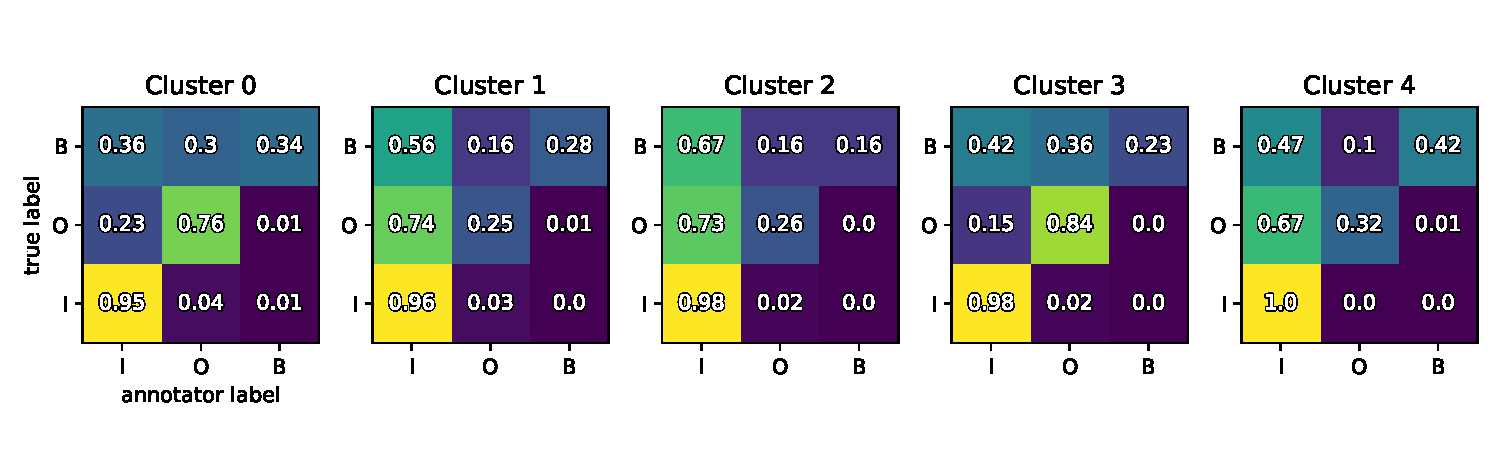
\includegraphics[width=0.88\textwidth, clip=True, trim=10 20 10 28]{figures/worker_models/seq_prev0_heatmap}
\vspace{0.2cm}
\\
\begin{minipage}[b][0.5cm][b]{0.1\textwidth} 
Previous label = O:\\
\vspace{1cm}
\end{minipage}
  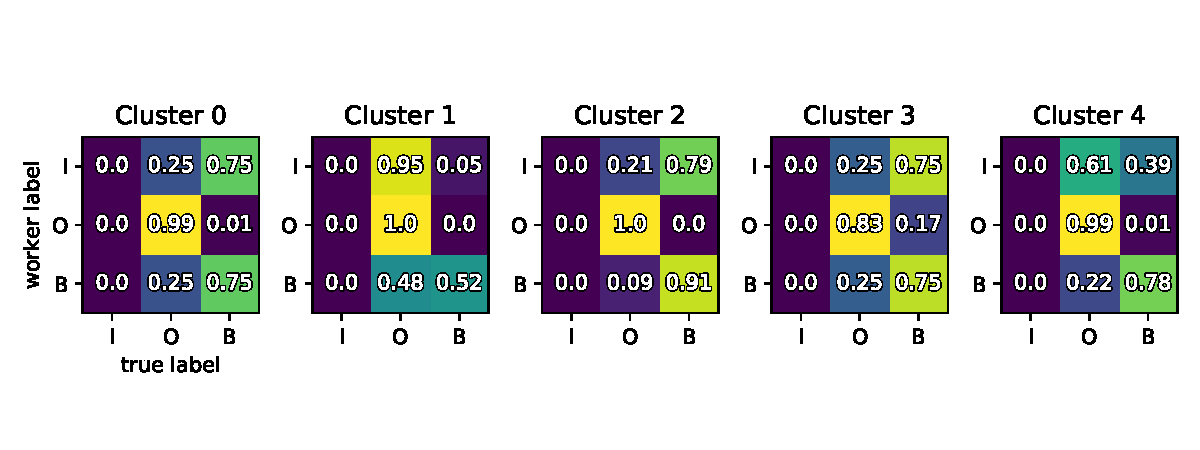
\includegraphics[width=0.88\textwidth, clip=True, trim=10 20 10 50]{figures/worker_models/seq_prev1_heatmap}
\vspace{0.2cm}
\\
\begin{minipage}[b][0.5cm][b]{0.1\textwidth} 
Previous label = B:\\
\vspace{1cm}
\end{minipage}
  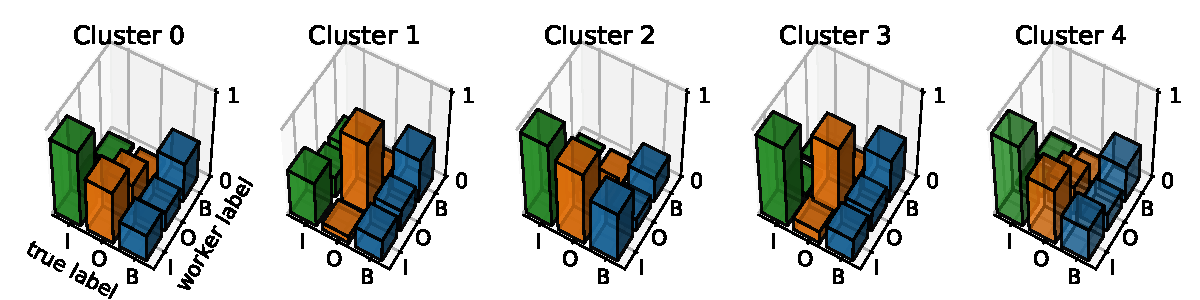
\includegraphics[width=0.88\textwidth, clip=True, trim=10 20 10 50]{figures/worker_models/seq_prev2_heatmap}
\\
\centering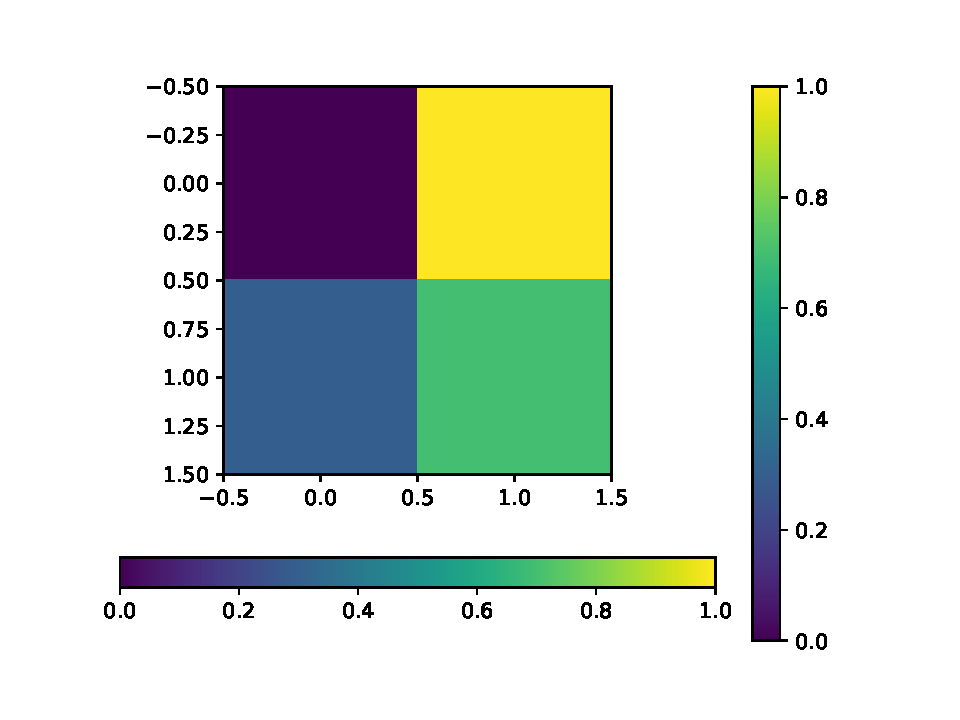
\includegraphics[width=0.45\textwidth,clip=True,trim=0 40 110 260]{figures/worker_models/colorbar}\\
\caption{Clusters of annotators in the PICO dataset. Each column shows the mean of the confusion matrices in the 
\textit{seq} annotator model for the members of one cluster, as inferred by BSC-seq.
 Each row corresponds to the mean confusion matrices conditioned on the annotator's previous label. 
 The confusion matrices are plotted as heatmaps,
where colours indicate the probabilities, which are also given by the numbers in each square.
}
\label{fig:conf_mat_clusters}
\end{figure*}
% TODO: make this plot more compact and relevant by plotting only the means across the whole dataset, 
%and the distribution of hellinger distances between the confusion matrices for each previous label case. Put on a single row.
%Table \ref{tab:aggregation_results} shows a benefit of using the sequential annotator model over CM, CV and acc.
\paragraph{Visualising Annotator Models. }
To determine whether, in practice, BSC-seq really learns distinctive confusion matrices depending on the previous labels,
we plot the learned annotator models for
PICO as probabilistic confusion matrices in Figure \ref{fig:conf_mat_clusters} (for an alternative visualisation, 
see Figure \ref{fig:anno_models_2} in the appendix).
%As the dataset contains a large number of annotators, we 
We clustered 
the confusion matrices % inferred by each model
into five groups by applying K-means to their posterior expected values,
then plotted the means for each cluster.
Each column in the figure shows the confusion matrices corresponding to the same cluster of annotators. 
In all clusters, BSC-seq learns different 
%accuracies for
confusion matrices depending on the previous label.
% B, I and O (the diagonal entries),
%which suggests that the data supports the use of this more complex model.
% explain ho
%These differences may explain its
%improvement over BSC-acc.
%BSC-CM differs from BSC-CV in that %has more distinctive clusters and 
%the first, fourth and fifth clusters 
%have off-diagonal values with different heights for the same true label value.
% The second 
%cluster for BSC-CM encodes likely spammers who usually choose 'O' regardless of the 
%ground truth. 
%Unlike BSC-CM, BSC-seq improved performance on PICO over BSC-CV. 
%The confusion matrices for BSC-seq are
%very different depending on the worker's previous annotation. 
There are also large variations between the clusters.
The third column, for example, shows
annotators with a tendency toward B$\Arrow{0.2cm}$I transitions regardless of the true label, while other clusters 
indicate very different labelling behaviour. The model therefore appears able to learn
distinct confusion matrices for different workers given previous labels, 
which supports the use of sequential
annotator models.

 \paragraph{Active Learning. }
 \begin{figure}[h]
 \centering
   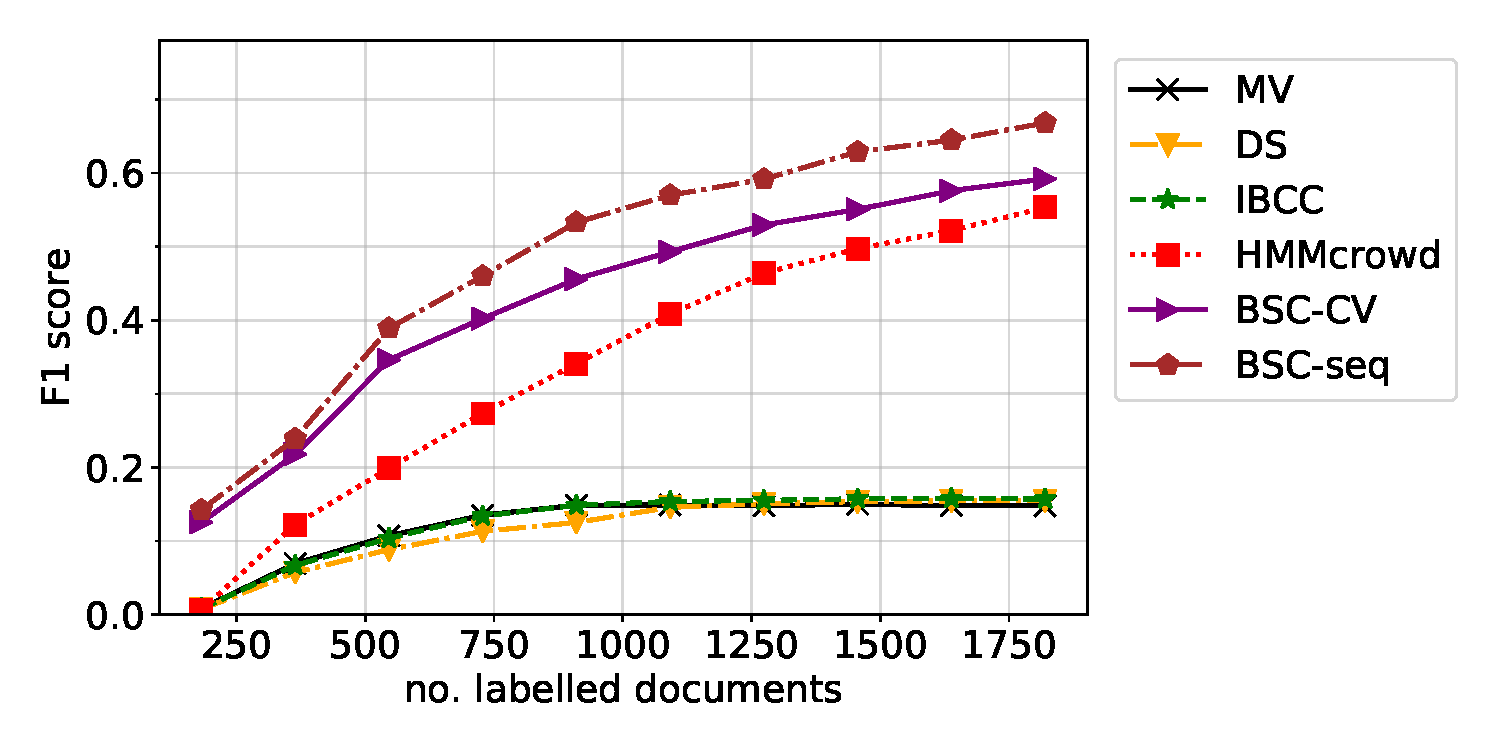
\includegraphics[width=0.3\columnwidth, clip=True, trim=530 160 20 20]{figures/NER_AL/pool/plot_F1-score.pdf}
      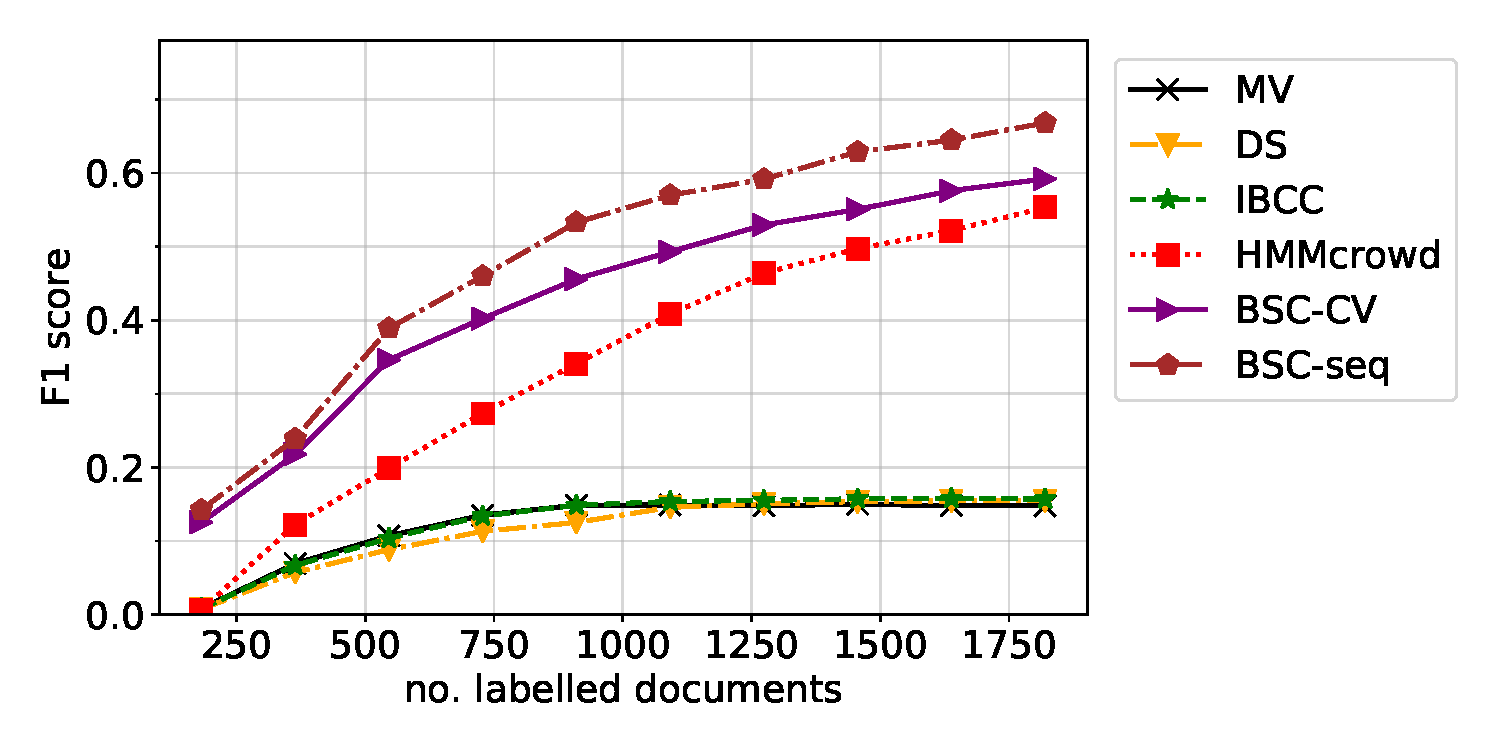
\includegraphics[width=0.9\columnwidth, clip=True, trim=40 22 190 15]{figures/NER_AL/pool/plot_F1-score.pdf}
 \caption{F1 scores for active learning simulations on NER using least-confidence 
 uncertainty sampling.
 %: prediction performance after each labelled batch is received. Mean scores over 10 repeats.
 }
 \label{fig:alner}
 \end{figure}
 Active learning is an iterative process that can reduce the amount of labelled
  data required to train a model.
  At each iteration, the active learning strategy selects informative data points,
  obtains their labels, 
  then re-trains a labelling model given the new labels.
 The updated model is then used in the next iteration to identify the most
 informative data points.  
 
  We simulate active learning in a crowdsourcing scenario
  where the goal is to learn the true labels,
  $\bs t$, by selecting documents for the crowd to label.
  Each document can be labelled multiple times by different workers.
  In contrast, in a passive learning setup, the number of annotations per document is 
  usually constant across all documents. 
  For example, in the PICO dataset, each
  document was labelled six times.
  The aim of active learning is to decrease the number of annotations required
  by avoiding relabelling documents whose true labels can be determined with  high confidence from fewer labels.
  
  We simulate active learning using 
 %a well-established technique, \emph{uncertainty sampling}
 the \emph{least confidence} strategy, shown to be effective by 
 ~\citet{settles2008analysis},
 as described in Algorithm \ref{al:uncertainty_sampling}.
At each iteration, we estimate $\bs t$ from the current set of 
  crowdsourced labels, $\bs c$,
  using one of the methods from 
  our previous experiments as the labelling model,
  then use this model to determine the least confident $batch\_size$ 
 documents to be labelled by the crowd. 
  If the simulation has requested all the labels for a document that
  are available in our dataset, this document is simply ignored when 
  choosing new batches
  and is not selected again.
 
 We hypothesise that BSC will learn more quickly than non-sequential 
 and non-Bayesian methods
 in the active learning simulation. 
 Bayesian methods such as BSC account for uncertainty in the model parameters when estimating confidence,  
 hence can be used to choose data points that rapidly improve
 the model itself.
 Sequential models such as BSC can also account for dependencies between sequence labels
 when estimating confidence.
% From the reviews:
%We apologise that the active learning experiment was not clear from the description. We use active learning to learn the aggregation models themselves, i.e. to train BSC-seq, BSC-CV, MV, etc. The F1-scores therefore evaluate the outputs of the aggregation models at each active learning round. The aim is to show how well each aggregation method performs on smaller numbers of annotations chosen by active learning. BSC-seq performs strongest, suggesting that using it with active learning could reduce the number of labels you need to obtain a desired F1 score for your aggregated labels. 
 %In contrast, frequentist methods
 %such as maximum likelihood output probabilities that do not account for parameter uncertainty due to 
 %small datasets or noisy labels. 
 
 %While various active learning methods could be applied here, in this paper we wish
 %to demonstrate only that BSC may serve as a good foundation for active learning,
 %and defer a deeper investigation of active learning techniques to future work.
 %TODO does there need to be another index in t for the document?
 \begin{algorithm}
 \DontPrintSemicolon
  \KwIn{ A random $initial\_set$ of training labels, the same for all methods. }
  \nl Set training set $\bs c=initial\_set$ \;
  \While{training set size $<max\_no\_labels$}
  {
  \nl Train model on $\bs c$ \;
  \nl For each document $n$, 
  compute $LC_n = 1-p(\bs t_n^*|\bs c)$, where $\bs t_n^*$ is the probability of the most likely sequence of labels 
  for $n$. \;
  \nl Obtain annotations for $batch\_size$ documents with the highest values of $LC$ (least confidence), and add them to $\bs c$\;
  }
 \caption{Active learning simulation using least-confidence sampling.}
 \label{al:uncertainty_sampling}
 \end{algorithm}
 
 Figure \ref{fig:alner} plots the mean F1 scores over ten repeats of the active learning simulation on the NER dataset (for clarity, we only plot key methods).
 When the number of iterations is very small, neither IBCC nor DS are able to outperform majority vote, and only produce a very small
 benefit as the number of labels grows. This highlights the need for a sequential model such as BSC or HMM-crowd for
 effective active learning with small numbers of labels.
 IBCC learns slightly quicker than DS,
 while BSC-CV clearly outperforms HMM-crowd: we believe this difference is due to the Bayesian treatment of IBCC and BSC,
 which means they are better able to estimate confidence than DS and HMM-crowd, which use maximum likelihood and maximum a posteriori inference.
 BSC-seq produces the best overall performance, and the gap grows as the number of labels increases, 
 since more data is required to learn the more complex annotator model.  
